
\subsection{研究背景}

\subsubsection{Radeon R600系列显卡命令处理机制}
Radeon R600显卡提供驱动使用命令流(Command Stream)的形式进行对显卡编程:驱动程序将需要对显卡进行配置的一连串命令写入命令缓冲区,写完之后进入让出处理器,显卡按照命令写入的顺序执行这些命令,执行完成后触发中断通知驱动。具体来说就是CPU将这些命令放入一个称为命令环的环形缓冲区中,命令环是GTT内存中分出来的一片内存,驱动程序往命令环中填充命令,填充完后通知GPU已经写入命令,接着GPU的命令处理器CP(Command Processor)接收并解析驱动程序发送过来的命令流,将解析后的数据传输给图形控制器的其他模块,包括3D图形处理器、2D图形处理器、视频处理器。

\begin{figure}[H] 
  \centering
  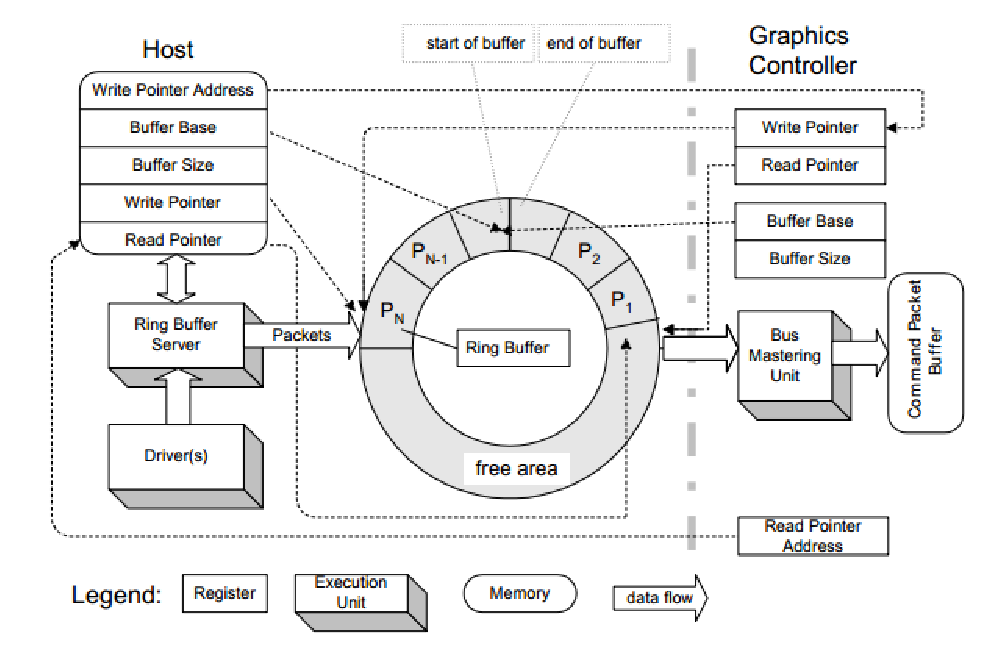
\includegraphics[width=16cm,height=12cm]{figures/chap03/CommandBuffer}
  \caption{Radeon R600系列显卡命令处理机制}
  \label{fig:CommandBuffer}
\end{figure}

如图\ref{fig:CommandBuffer},左边的Host(CPU)和右边的GPU各自记录了命令环的起始地址,并各自保存了一份读写指针,CPU写之前首先查询读指针,确认有空闲空间之后写入内容并更新写指针,GPU读取了命令之后更新读指针。CPU和GPU都要共同维护和管理环形缓冲区的状态:基地址、长度、写指针和读指针。为了使Ring Buffer能够正常工作,CPU和GPU必须维护这种状态的一致性。Ring Buffer基地址和大小是在系统第一次启动时已经初始化好的,之后一般也不会改变。当操作Ring Buffer时, 读指针和写指针的修改非常频繁。为了维护环形缓冲区的状态一致性,当写操作者(CPU)更新写指针时,它必须将写指针告诉GPU。同样的,当读操作者(GPU)更新读指针时,它必须将读指针告知CPU。无论是CPU还是GPU都是从低地址开始进行填写或抽取操作的,一旦到了环形缓冲区的结束处,又从环形缓冲区起始处继续\cite{Radeon-Manual}。  

上面提到的Radeon显卡命令是以命令包的形式出现的,如今Radeon系列显卡有4中命令包,分别是0型、1型、2型和3型命令包,命令包由两部分组成,第一部分是命令包头,第二部分是命令包主体,命令包头为请求GPU执行的具体操作,命令主体为执行该操作需要的数据。

下面分别介绍一下这四种命令包:

\begin{itemize}

\item{\textbf{0型命令包}} \\
0型命令包用于写连续N个寄存器。包主体部分是依次往这些寄存器写的值。包头各个部分的意义为:
\vspace{6pt}
\begin{center} \tablecaption{0型命令包 \label{tab:0-command}} 
\tablefirsthead{
\rowcolor[gray]{0.8}
\multicolumn{1}{l}{\textbf{位}} &
\multicolumn{1}{l}{\textbf{域名称}} &
\multicolumn{1}{c}{\textbf{描述}} \\ }
\tablehead{\multicolumn{3}{c}{
\small 表 \ref{tab:0-command} (续) } \\
\rowcolor[gray]{0.8}
\multicolumn{1}{l}{\textbf{位}} &
\multicolumn{1}{l}{\textbf{域名称}} &
\multicolumn{1}{c}{\textbf{描述}} \\ }
\tabletail{\bottomrule
\multicolumn{3}{c}{\small 接下页} \\}
\tablelasttail{\bottomrule}

\begin{supertabular}{p{2.cm}p{3.cm}m{10.cm}}
	12:0 & BASE\underline{ }INDEX & 要写的连续寄存器的第一个寄存器地址,最大地址0x7FFF \\
	14:13 & 保留位 & \\
	15 & ONE\underline{ }REG\underline{ }WR &  \\ 
	& & \tabitem 0表示将包主体的数据依次写入寄存器中 \\
	& & \tabitem 1表示所有数据写入同一个寄存器 \\
	29:16 & COUNT & 要写的寄存器数目N-1 \\
	31:30 & TYPE & 包类型,0型命令包类型名为0 \\
\end{supertabular}
\end{center}
\vspace{6pt}


\item{\textbf{1型命令包}} \\
1型命令包用于写两个的寄存器,1型命令包包头定义如下:
\vspace{6pt}
\begin{center} \tablecaption{1型命令包 \label{tab:1-command}} 
\tablefirsthead{
\rowcolor[gray]{0.8}
\multicolumn{1}{l}{\textbf{位}} &
\multicolumn{1}{l}{\textbf{域名称}} &
\multicolumn{1}{c}{\textbf{描述}} \\ }
\tablehead{\multicolumn{3}{c}{
\small 表 \ref{tab:1-command} (续) } \\
\rowcolor[gray]{0.8}
\multicolumn{1}{l}{\textbf{位}} &
\multicolumn{1}{l}{\textbf{域名称}} &
\multicolumn{1}{c}{\textbf{描述}} \\ }
\tabletail{\bottomrule
\multicolumn{3}{c}{\small 接下页} \\}
\tablelasttail{\bottomrule}

\begin{supertabular}{p{2.cm}p{3.cm}m{10.cm}}
	10:0 & REG\underline{ }INDEX1 & 第一个寄存器的地址 \\
	22:11 & REG\underline{ }INDEX2 & 第二个寄存器的地址 \\
	29:22 & RESERVED & 保留位 \\
	31:30 & TYPE & 1型命令包的类型为0x1 \\
\end{supertabular}
\end{center}
\vspace{6pt}

\item{\textbf{2型命令包}} \\
2型命令包是一个空命令包,用于填充对齐命令。2型命令包没有包主体,其包头最高两位为0x2,其它位无意义。

\item{\textbf{3型命令包}} \\
3型命令包是最功能最丰富的包,图形的主要功能都是通过这类包实现的。3型命令包主体内容由包头的IT\underline{ }OPCODE决定。3型命令是主要的命令包,涵盖了寄存器设置/绘图命令/同步等主要操作。3型命令包包头定义如下:
\vspace{6pt}
\begin{center} \tablecaption{3型命令包 \label{tab:3-command}} 
\tablefirsthead{
\rowcolor[gray]{0.8}
\multicolumn{1}{l}{\textbf{位}} &
\multicolumn{1}{l}{\textbf{域名称}} &
\multicolumn{1}{c}{\textbf{描述}} \\ }
\tablehead{\multicolumn{3}{c}{
\small 表 \ref{tab:3-command} (续) } \\
\rowcolor[gray]{0.8}
\multicolumn{1}{l}{\textbf{位}} &
\multicolumn{1}{l}{\textbf{域名称}} &
\multicolumn{1}{c}{\textbf{描述}} \\ }
\tabletail{\bottomrule
\multicolumn{3}{c}{\small 接下页} \\}
\tablelasttail{\bottomrule}

\begin{supertabular}{p{2.cm}p{3.cm}m{10.cm}}
	7:0 & reserved & 保留位 \\
	15:8 & IT\underline{ }OPCODE & 操作码 \\
	29:16 & COUNT & 包主题DWORDS数目-1 \\
	31:30 & TYPE & 3型包类型为0x3 \\
\end{supertabular}
\end{center}
\vspace{6pt}
\end{itemize}

\subsubsection{Mesa3D显示列表绘制模式实现原理}
\label{sec:display-list}

显示列表绘制模式即glGenList/glNewList/glEndList/glCallList,它可以提高性能,因为它存储OPENGL的函数,供以后使用,如果需要多次重绘同一个几何图形,或者如果一次需要多次调用的用于更改状态的函数,把这些函数存储在显示列表中,此时将显示列表中的矩阵结果集保存,后续使用不需要重复计算以提高性能。显示列表更像是命令缓存器,而不是动态数据库,也就是说当显示列表创建后,就无法修改。同时显示列表的创建也存在一定的系统开销,因此一个小的显示列表未必会提升性能。

我们以下面所示的svPerfGL测试集里面的显示列表模式为例,来看一下Mesa3D图形库是如何实现显示列表的绘制模式的。

\begin{lstlisting}
 // Create Display List
 glNewList(trianglesListIndx, GL_COMPILE);
 glDrawArrays(GL_TRIANGLES, 0, tNumVerts);
 glEndList(); 

 // Call Display List
 glCallList(trianglesListIndx);
\end{lstlisting}


当执行glNewList时,Mesa3D图形库会执行alloc\underline{ }vertex\underline{ }store函数预分配大小为VBO\underline{ }SAVE\underline{ }BUFFER\underline{ }SIZE*sizeof(GLfloat)的空白VRAM空间,这个空间我们姑且称之为buffer0。在显示列表机制下,保存模式的glDrawArrays只会执行一次,目的是将所有的顶点属性(位置、法线和颜色等)写入buffer0。VBO\underline{ }SAVE\underline{ }BUFFER\underline{ }SIZE的初值是8*1024,只能存放8*1024/3=2730个顶点属性,而glDrawArrays可能需要写入更多的顶点属性,因此buffer0是远远不够存放这些顶点属性的。当buffer0溢出后,显示列表会继续分配大小为VBO\underline{ }SAVE\underline{ }BUFFER\underline{ }SIZE * sizeof(GLfloat)的buffer1,buffer2,buffer3...直到所有顶点属性都写入VRAM。可见,当glDrawArray执行完时,所有的顶点属性已经存入VRAM,但是分散在很多个小buffer中。

接着通过执行glCallList来调用已保存好顶点属性的显示列表,glCallList将执行vbo\underline{ }save\underline{ }playback\underline{ }vertex\underline{ }list函数来实现渲染,该函数调用r600\underline{ }draw\underline{ }vbo向GPU发如下命令:

\begin{lstlisting}
cs->buf[cs->cdw++] = PKT3(PKT3_DRAW_INDEX_AUTO, 1, 
                          rctx->predicate_drawing);
cs->buf[cs->cdw++] = info.count;
cs->buf[cs->cdw++] = V_0287F0_DI_SRC_SEL_AUTO_INDEX 
                     | (info.count_from_stream_output? 
                        S_0287F0_USE_OPAQUE(1) : 0);
\end{lstlisting}

这些命令通过Command Stream机制被GPU读取并执行,从而启动pipeline进行3D渲染。

\begin{figure}[H] 
  \centering
  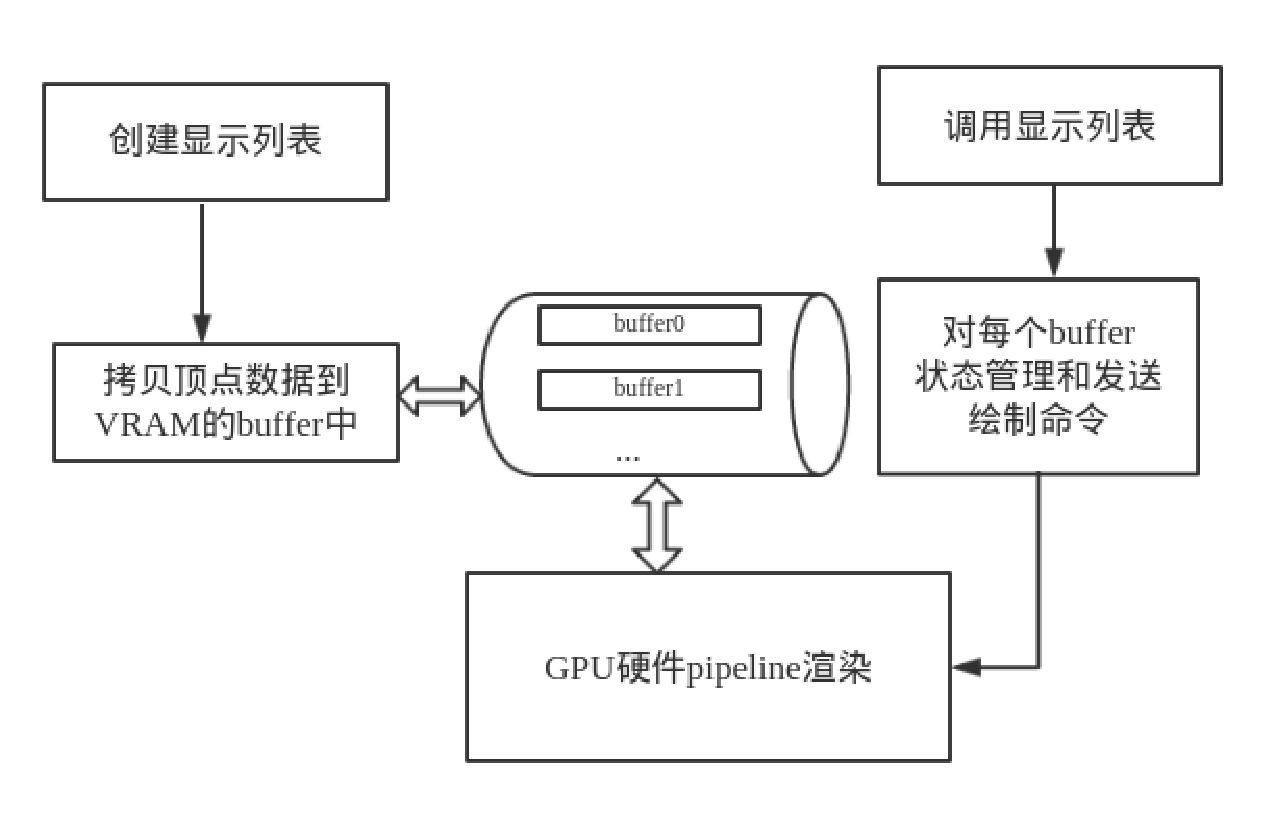
\includegraphics[width=12cm,height=10cm]{figures/chap03/display-list-flow}
  \caption{Mesa3D图形库显示列表实现机制}
  \label{fig:display-list-flow}
\end{figure}

由于显示列表是一次创建多次调用,所以如图\ref{fig:display-list-flow}所示,每次在调用显示列表时候都会做对每个buffer进行状态管理和发送绘制命令到GPU。GPU在执行完3D渲染之后将结果放入framebuffer中然后通过显示设备显示出来。

\subsection{CPU与GPU负载分析}

我们在前面就介绍过Radeon R600系列GPU的工作模型就是CPU端将数据和命令写入Command Buffer中,然后GPU读取Command Buffer中的命令并执行(图\ref{fig:CommandBuffer})。所以从这个模型我们可以看到这里存在着CPU/GPU的负载平衡问题:如果CPU端执行效率比GPU端执行效率更快,那么会导致Command Buffer满载,这样CPU就不得不需要同步操作停下来等待GPU处理完命令以得到Command Buffer里面一些空闲的位置继续写入命令;同样,如果GPU端执行的效率更高,这样每当CPU写完命令之后GPU就可以很快的执行完毕,这样Command Buffer常常会处于空闲状态,GPU就不得不空闲下来等待CPU的处理结果。不论是哪一种情况都属于CPU与GPU的负载不平衡,这样都会造成性能的瓶颈。

从前面的分析里面我们可以知道显示列表模式的CPU和GPU的协同工作模型就是:CPU数据准备与状态管理、GPU处理数据、CPU数据准备与状态管理、GPU处理数据、反复直至数据全部处理完毕。那么现在我们就从CPU与GPU的负载平衡的关系上来看我们将上面提到的svPerfGL里面的显示列表模式测试项的情况。这里测试每帧100万个三角形的绘制时候CPU和GPU的负载状况。测试结果如下图\ref{fig:cpu-load-dsp}和图\ref{fig:gpu-load-dsp}

\begin{figure}[H]
  \begin{minipage}[t]{0.5\linewidth} 
  \centering
  \includegraphics[width=8cm,height=6cm]{figures/gnuplot/dsp/cpu-load}
  \caption{显示列表测试项CPU负载}
  \label{fig:cpu-load-dsp}
  \end{minipage}
  \begin{minipage}[t]{0.5\linewidth} 
  \centering
  \includegraphics[width=8cm,height=6cm]{figures/gnuplot/dsp/gpu-load}
  \caption{显示列表测试项GPU负载}
  \label{fig:gpu-load-dsp}
  \end{minipage}
\end{figure}

从上面的图中我们可以看到CPU的负载情况明显比GPU要大很多,这里的原因也很好解释: 如前面章节\ref{sec:display-list}研究的那样,对每一次的buffer,Mesa3D需要都先在CPU端数据准备和状态管理,然后提交给GPU处理。这里当我们绘制大量的顶点时候,例如glDrawArray函数里面写入100万个三角形,那么每个三角形需要有3个顶点*3钟顶点属性(位置、法线和颜色),所以一种有1000000*3*3即9000000个顶点属性,根据前面分析的默认的buffer大小是8*1024*4字节,那么总共需要的buffer数目就是9000000*3*4/(8*1024*4)即3296个。由于对这3296个buffer每一个都需要CPU进行进行数据准备和状态管理等大量操作,这对性能较为优越的X86不是问题,却能极大的消耗龙芯3A的CPU。这样也就造成了CPU负载过大,而GPU负载较小的结果。


\subsection{CPU与GPU负载平衡优化}

由前一节分析我们可以看到CPU负载过大导致了CPU与GPU负载不平衡问题,究其原因就是CPU端需要处理的buffer数目过多,于是本文提出了一种通过调整显示列表缓存buffer大小的方法来优化显示列表的CPU与GPU负载不平衡问题。

如前面章节\ref{sec:display-list}所分析的那样,显示列表由于数据都已经上传保存到VRAM中的buffer里面,所以每次调用显示列表时候并不需要再次上传数据,而只是对每个buffer进行数据准备和状态管理即可,这些工作与buffer所装载的数据大小并没有关系,于是我们可以将buffer的大小调整到一个合适的数值,然后使得CPU的负载降低,GPU的负载增加以提高整体性能。

为了寻找显示列表缓存buffer的合适大小,我们通过测试svPerfGL显示列表程序在60秒内绘制每帧100万个三角形的绘制性能来确定这一合适值。相关测试结果如下表\ref{tab:buffer-performance}:

\begin{center} \tablecaption{svPerfGL显示列表测试项不同buffer大小下绘制性能 \label{tab:buffer-performance}} 
\tablefirsthead{
\rowcolor[gray]{0.8}
\multicolumn{1}{c}{\textbf{buffer大小}} &
\multicolumn{1}{c}{\textbf{帧数}} &
\multicolumn{1}{c}{\textbf{渲染效率(frame/s)}} \\ }
\tablehead{\multicolumn{3}{c}{
\small 表 \ref{tab:0-command} (续) } \\
\rowcolor[gray]{0.8}
\multicolumn{1}{c}{\textbf{buffer大小}} &
\multicolumn{1}{c}{\textbf{帧数}} &
\multicolumn{1}{c}{\textbf{渲染效率(frame/s)}} \\ }
\tabletail{\bottomrule
\multicolumn{3}{c}{\small 接下页} \\}
\tablelasttail{\bottomrule}

%./svPerfGL -i ../../trisNormsColors-512.nc -w 1280 -h 1024 -2 -r -t 60 -s 3000000
\begin{supertabular}{p{6.cm}p{3.cm}m{6.cm}}
	32K& 169& 2.81\\
	64K& 250& 4.16\\
	128K& 241& 4.01\\
	256K& 242& 4.03\\
	512K& 266& 4.42\\
	1024K& 268& 4.46\\
	2048K& 269& 4.47\\
	4096K& 209& 3.47\\
\end{supertabular}
\end{center}

根据测试结果,我们可以发现将buffer的大小设定为2048KB能够取得较好的性能。此时再次测量CPU和GPU的负载状况如图\ref{fig:cpu-load-dsp-opt}和图\ref{fig:gpu-load-dsp-opt}:

\begin{figure}[H] 
  \begin{minipage}[t]{0.5\linewidth} 
  \centering
  \includegraphics[width=8cm,height=6cm]{figures/gnuplot/dsp/cpu-load-opt}
  \caption{显示列表测试项优化后CPU负载}
  \label{fig:cpu-load-dsp-opt}
  \end{minipage}
  \begin{minipage}[t]{0.5\linewidth} 
  \centering
  \includegraphics[width=8cm,height=6cm]{figures/gnuplot/dsp/gpu-load-opt}
  \caption{显示列表测试项优化后GPU负载}
  \label{fig:gpu-load-dsp-opt}
  \end{minipage}
\end{figure}

可以看到此时GPU刚好达到了满载,CPU负载较轻,因为龙芯平台CPU处理能力较GPU的处理能力稍弱,所以这样的负载关系比较符合当前硬件特点,所以能够取得较好的性能提升。

当然buffer大小调整这种优化方法也有一定的缺点,我们将buffer的大小调大的时候会增加VRAM的管理粒度,在小数据规模时候可能会造成VRAM的浪费,特别是在某些显卡显存比较紧俏的机器环境下可能会消耗掉所有的VRAM空间,造成VRAM空间不够程序无法执行的问题。所以这个优化方法可以作为可配置的优化手段,在实际工程应用中可以根据具体硬件情况进行选择。
